\section{Технический проект}
\subsection{Общая характеристика организации решения задачи}

Необходимо спроектировать и разработать приложение, с помощью которого можно редактировать различные изображения.

Графический редактор представляет собой программное средство, разработанное для создания, редактирования и обработки графических изображений. Он предоставляет пользователю набор инструментов и функций для работы с различными видами графики, включая рисунки, фотографии, иллюстрации и другие визуальные материалы.

\subsection{Обоснование выбора технологии проектирования}

На сегодняшний день информационный рынок, поставляющий программные решения в выбранной сфере, предлагает множество продуктов, позволяющих достигнуть поставленной цели – разработки графического редактора.

\subsubsection{Описание используемых технологий и языков программирования}

В процессе разработки графического редактора используются программные средства и языки программирования. Каждое программное средство применяется для круга задач, при решении которых оно необходимо.

\subsubsection{Язык программирования Python}

Python — высокоуровневый язык программирования общего назначения с динамической строгой типизацией и автоматическим управлением памятью, ориентированный на повышение производительности разработчика, читаемости кода и его качества, а также на обеспечение переносимости написанных на нём программ.

\paragraph{Достоинства языка Python}

Простота и читаемость: Python известен своей простотой синтаксиса, что делает его легким для изучения и понимания. Читаемый код способствует совместной работе и обслуживанию.

Множество библиотек и фреймворков: Python обладает обширным экосистемой библиотек и фреймворков, что упрощает разработку приложений в различных областях, таких как веб-разработка, научные вычисления, машинное обучение и другие.

Портативность: Python поддерживает множество платформ, что позволяет запускать программы на различных операционных системах без изменений в коде.

\paragraph{Недостатки языка Python}

Производительность в некоторых случаях: В сравнении с некоторыми компилируемыми языками, Python может быть менее производительным, особенно в задачах, требующих высокой вычислительной мощности.

Глобальная блокировка интерпретатора (GIL): GIL ограничивает одновременное выполнение нескольких потоков в Python, что может быть проблемой в многопоточных приложениях.

Объем занимаемой памяти: Python может потреблять больше памяти по сравнению с некоторыми другими языками.

\subsection{Диаграмма компонентов и схема обмена данными между файлами компонента}

Диаграмма компонентов описывает особенности физического представления разрабатываемого приложения. Она позволяет определить архитектуру системы, установив зависимости между программными компонентами, в роли которых может выступать как исходный, так и исполняемый код. Основными графическими элементами диаграммы компонентов являются компоненты, интерфейсы, а также зависимости между ними. На рисунке \ref{compo:image} изображена диаграмма компонентов для проектируемого приложения. Она включает в себя начальное и основное окно, в котором находятся компоненты «Холст» и «Инструмент». Инструментом может быть: кисть, карандаш или ластик.

\begin{figure}[ht]
\center{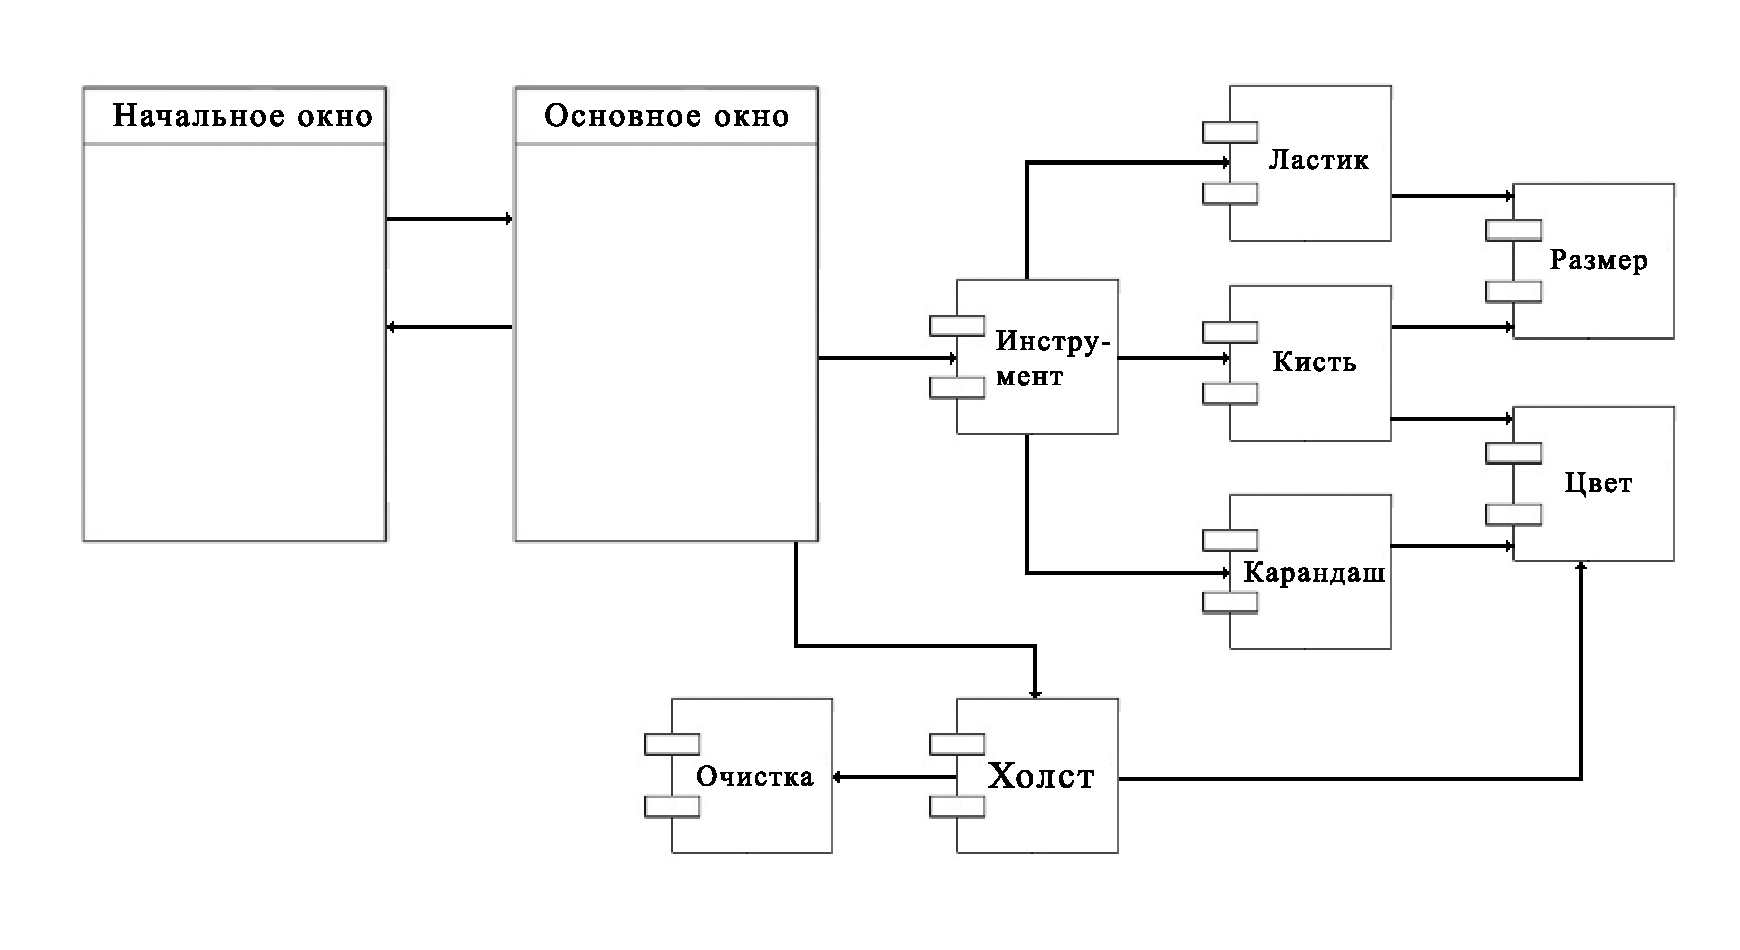
\includegraphics[width=1\linewidth]{compo}}
\caption{Диаграмма компонентов}
\label{compo:image}
\end{figure}

Любой компонент должен быть вызван в сценарии редактора. Редактор передает данные компоненту в момент вызова последнего.

На рисунке \ref{cp2:image} представлена схема обмена данными между сценариями редактора при взаимодействии компонентов.

\begin{figure}[ht]
\center{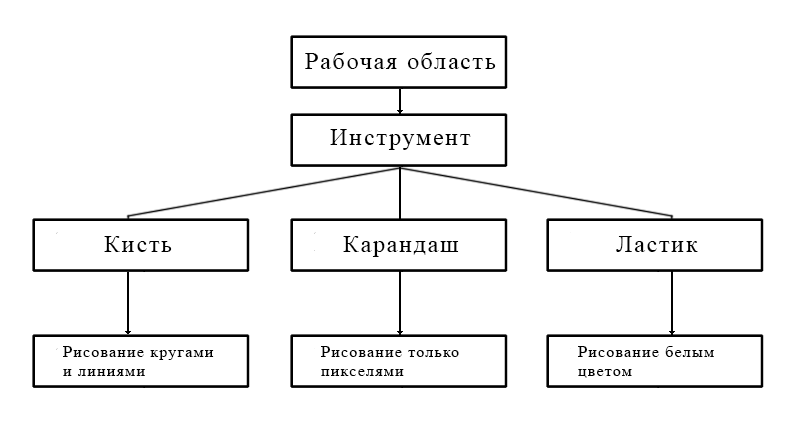
\includegraphics[width=1\linewidth]{cp2}}
\caption{Диаграмма компонентов}
\label{cp2:image}
\end{figure}

При взаимодействии с компонентом в сценарии редактора происходит распознавание взаимодействующих объектов.
Если пользователь выберет объект «Кисть», то он перейдет в обычный режим рисования. Нажатием левой кнопки мыши, он будет создавать круги, которые соединяются между собой линиями. Если пользователь выберет объект «Карандаш», то он перейдет в режим рисования пикселями. Взаимодействие с рабочей зоной будет создавать на ней единичные пиксели. Если пользователь выберет объект «Ластик», то он сменит цвет своей кисти на белый.

Работа компонента заканчивается в момент завершения работы сценария редактора.

\subsection{Содержание информационных блоков. Основные сущности}

Проанализировав требования, можно выделить одну основную сущность:
\begin{itemize}
\item "<Кисточка">;
\end{itemize}

В состав сущности "<Кисточка"> можно включить атрибуты, представленные в таблице \ref{news:table}.

\begin{xltabular}{\textwidth}{|l|l|p{1.7cm}|X|}
	\caption{Атрибуты сущности "<Кисточка">\label{news:table}}\\ \hline
	\centrow Поле & \centrow Тип & \centrow Обяза\-тельное & \centrow Описание \\ \hline
	\thead{1} & \thead{2} & \centrow 3 & \centrow 4 \\ \hline
	\endfirsthead
	\continuecaption{Продолжение таблицы \ref{news:table}}
	\thead{1} & \thead{2} & \centrow 3 & \centrow 4 \\ \hline
	\finishhead
	color & str & true & Цвет кисти \\ \hline 
	brush\_size & int & true & Размер кисти \\ \hline 
	lcolor & str & false & Предыдущий цвет кисти \\ \hline 
	pixel\_flag & bool & true & Тип кисти \\ \hline 
	lx & list & true & Список x координат кисти \\ \hline 
	ly & list & true & Список y координат кисти
\end{xltabular}


